\documentclass[UTF8,11pt,a4paper]{ctexart}
\usepackage{hyperref}
\usepackage{amsmath}
\usepackage{geometry}
\usepackage{ulem}
\usepackage{multirow}
\usepackage{color}
\usepackage{fontspec}
\usepackage{graphicx}
\usepackage{amsfonts}
\usepackage{amssymb}
\usepackage{booktabs}
\usepackage{fancyhdr}

\geometry{left=2cm,right=2cm,top=2cm,bottom=2.0cm}
\title{\textbf{高三生存指南}}

\author{武汉大学 wjyyy}

\pagestyle{fancy}

\fancyhead[L]{高三生存指南}
\fancyhead[R]{wjyyy}
\fancyfoot[C]{第 \thepage 页,共 9 页}

\setmonofont{Consolas}

\begin{document}
	\maketitle
	\tableofcontents
	\section{高三概况}
		高三一年,你会如同一个学习机器一样,每天从早学到晚,任何放松都可能会使你感到罪恶。用郦道元的一句环境描写借景抒情就是:
		\begin{quote}
			\textit{自非亭午夜分,不见曦月。}
			\flushright\textit{——郦道元《三峡》}
		\end{quote}
		
		高三会有各种名目的考试,从强化训练、日常考试、周考、月考、联考、调考……直到高考。总会有订正不完的错题、分析不完的试卷以及出其不意的新题型、新概念。
		
		刚上高三的时候,会面对一轮复习,持续约4个月,接着有二轮三轮复习。如果高一高二不是很努力,不用担心,多轮的高效复习会帮助你查漏补缺,但是必须付出一些高一高二没有付出的时间和精力。
		
		高三的寒假是绝佳的弯道超车机会,因为它为你提供了足够的时间来做题、落实、总结。
		
		高考前,学校会组织多次适应性考试,来让考生适应高考的氛围。就我而言,与其说是适应高考,还不如说是在让学生对高考的紧张感到麻木,不再紧张地踏上高考考场。
		
		\begin{quote}
			\textit{哎呀,又周二了,背会书去考试。}
			\flushright\textit{——wjyyy于2020年7月7日}
		\end{quote}
	
		因为2020年的高考是周二周三,所以6月的每个周二周三,学校都组织了高质量的周考。5周以后,我们已经养成了周二参加周考的“习惯”。
		
		高考结束后14天,可以通过准考证上提供的途径查询分数,随后可以填报志愿。
	\section{高三建议 - 方法}
		\subsection{听课}
			听课时需要认真,但没必要全神贯注。一定程度的认真可以使你不错过老师的授课重点,而过于认真会让人感到无聊和困倦。
			
			保持认真的方式有:跟随老师互动、记笔记、树立知识框架等。
			\subsubsection{跟随老师互动}
				跟随老师互动看上去可能有些距离感,但是实际上只需要回答老师向大家提出的问题,在老师解释问题的时候点一下头或者用眼神、表情等与老师传递信息。这样老师可以大致了解听讲的效果,及时补充可能没有讲清楚的问题,并调整讲课的节奏,适当推进较为简单的内容。
				
				举个例子:
				
				\begin{quote}
					老师:我们之前是不是学过圆的标准方程 $x^2+y^2=r^2$?
					
					\texttt{情况1:}
					
					学生:是/(点头)
					
					老师:那么类似地,椭圆也有 $\frac{x^2}{a^2}+\frac{y^2}{b^2}=1$ 的标准方程。
					
					\texttt{情况2:}
					
					学生:嗯?/(沉默)/(迷茫)
					
					老师:好,我再给大家复习一下圆的标准方程。
					
				\end{quote}
			
				这样就有可能有效避免“跟不上”的情况。
			\subsubsection{记笔记}
				记笔记一定程度上是为了复习,所以排版尽可能工整。
				
				一般老师在黑板上写的是提纲,有助于你的\textbf{初步排版和建立知识框架}。老师写在黑板上的东西都是要记在笔记本上的,而老师所讲的我们要选择性记在本子上。
				
				事实上,由于记笔记,我们的思路就不由自主地跟上了老师。没有记笔记的时候也可以拿笔在草稿纸上把听到的、想到的写写画画,也有助于紧跟老师。
				
				而我们记笔记的时候需要稍微思考一下,不能只动手不动脑。思考时不仅可以帮助理解知识点,还可以悄然记住知识点在笔记本上的位置,写作业、复习时通过笔记本查找信息时会比较方便。
				
				此外,记笔记可以用多种颜色的笔。最基础的是\textbf{黑、{\color{red}红}、{\color{blue}蓝}}三种。
				
				\begin{figure}[h]
					\centering
					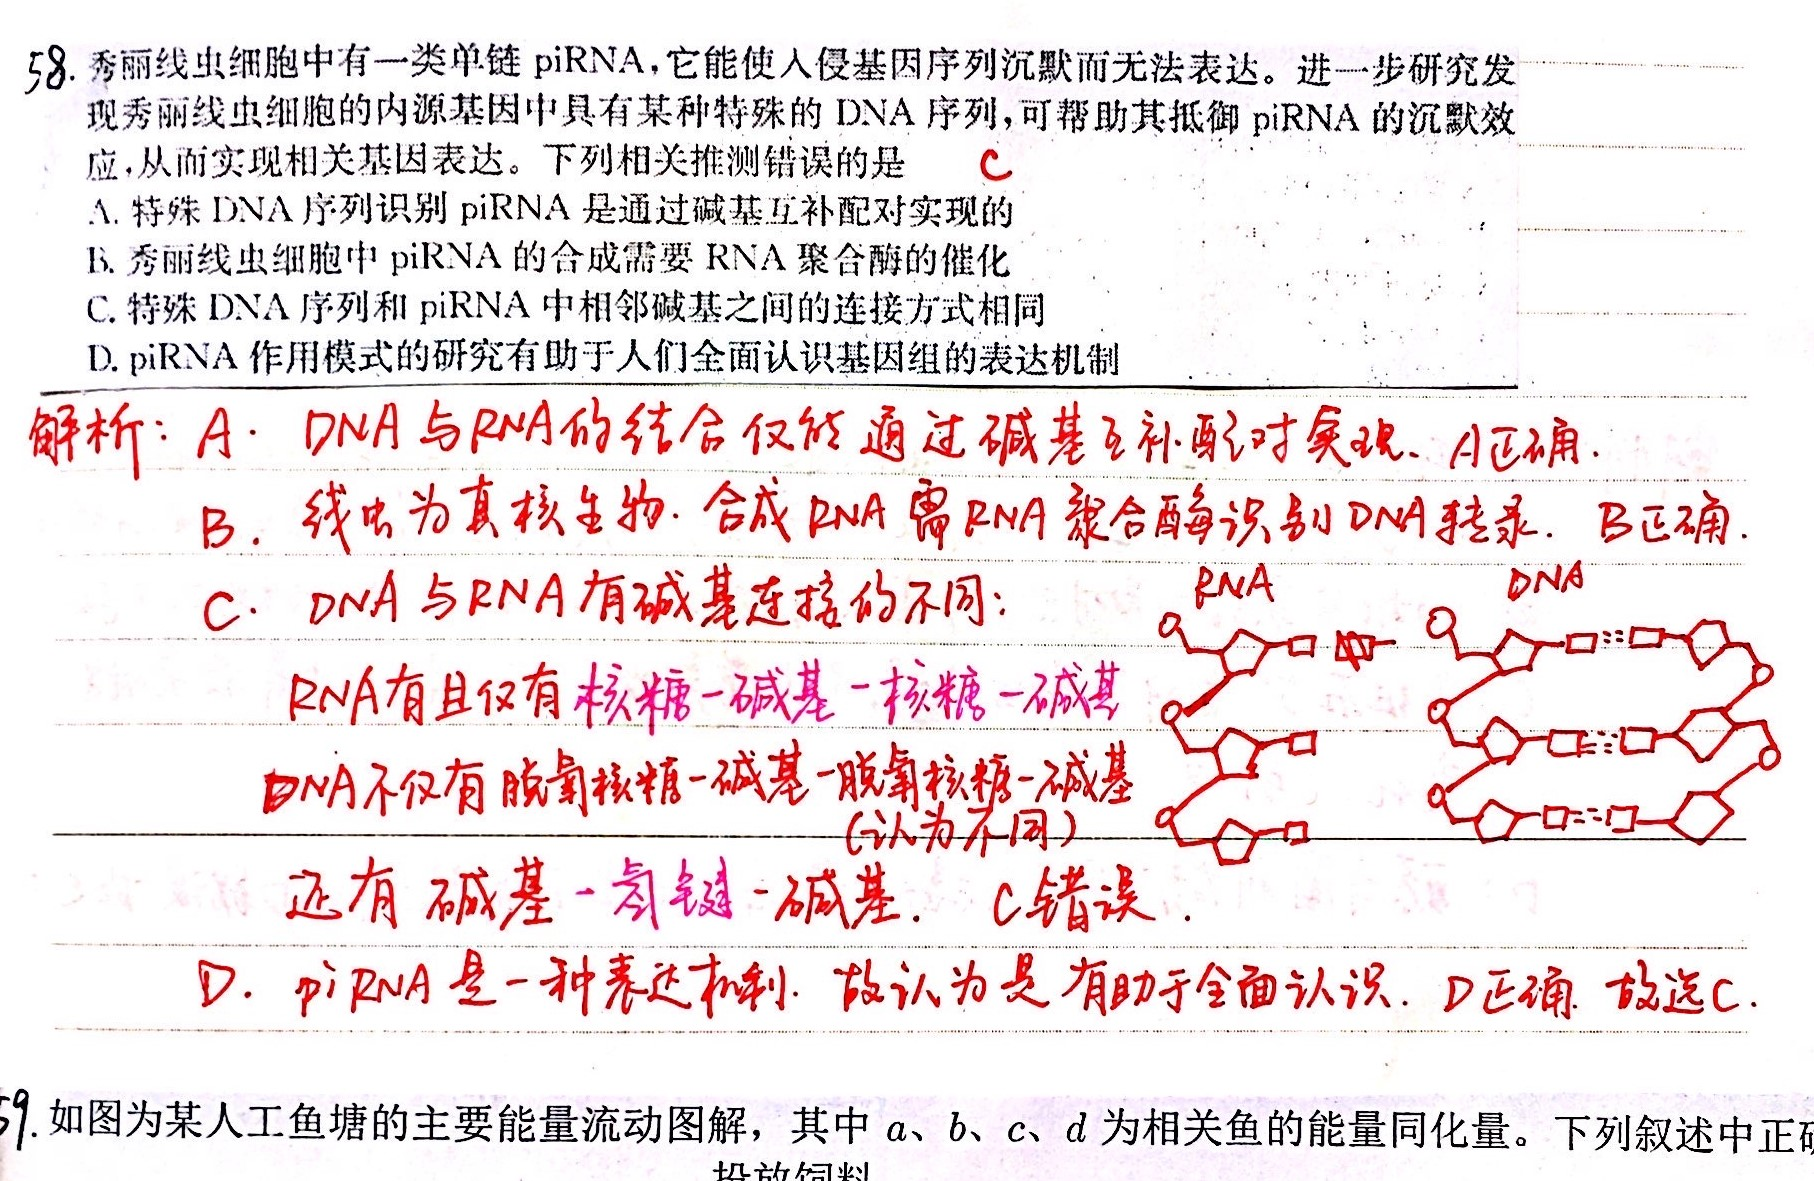
\includegraphics[width=14cm,height=10cm]{IMG_3110.JPG}
					
					\caption{三色笔记示例图({\color{red}红}黑{\color{magenta}紫})}
				\end{figure}
			\subsubsection{树立知识框架}
				在学习过程中有知识框架后,你就可以知道当前所学的知识建立在哪些知识的基础上,有了整体的一个俯瞰,学习过程就不会那么枯燥了。
		\subsection{与同学的互动}
			高三与同学的互动主要是下课聊天、结伴,吃饭打水,住寝室等。只要正常交流,都不会影响同学关系。和睦的同学关系有助于维持良好的心情,从而提升成绩。
			\subsubsection{班干部}
				班干部会牺牲一部分时间去开会或处理事情,这就要求班干部们预算好写作业的时间。虽然班干部需要较强的时间管理能力,但是更容易和同学们打好交道。
			\subsubsection{课代表}
				课代表是直面老师的群体,可以与老师近距离交流,获得相对更多的指导。而有时提交的作业量和ddl\footnote{ddl:deadline的缩写。deadline:最后期限。}掌握在课代表手里,完成作业的自由度变高了。
		\subsection{改错本}
			改错本是高中学习相当重要的一环。它可以促进你对错题的重做、消化和落实。当然,自己及时更新改错本比老师催更改错本的效果要好几倍。
			\subsubsection{改错本的要素}
				首先需要有题目、正确答案、分析过程。题目可以在老师的允许下裁剪试卷,正确答案建议自己重新认真写过程,分析过程是对正确答案步骤的解释,有助于复习时的思路清晰。
				
				当然,有些老师为保留试卷的完整性,需要同学们保存好试卷,这样的话,题目就只能复印或者誊抄了。
				
				除了以上提到的,还有其他要素可以加入。比如题目来源、题号、登记时间等,一方面可以记录下改错本的进度,获得更多的成就感;另一方面也可以剖析试卷的组成情况,更加了解试卷及相应考试,做起来更得心应手。
				
				比方说,2019年11月2日,改错本上收集了一道高三年级七校联考物理25题。而在第二次七校联考时,看到这个题目就可以考虑本次考试的备考重点和查漏补缺的方向。
			\subsubsection{改错本的用法}
				首先在考试前可以看改错本的错题,了解自己思想和能力上的薄弱点。其次,平时在遇到相同知识点的瓶颈时可以用来复习巩固知识。甚至还可以练习解题的速度。
				
				同时,工整的抄写和画图可以练字和提升动手能力,也可以对题目中的情景有更深的理解。
				
				{\color[gray]{0.6}同理,当一个东西记不住时,多抄几遍就能记住了。}
				
				最好是做到错一次并改正,以后这样的题就不再错了。
		\subsection{其他技能}
			考试技巧比较重要的一点是揣摩命题人意图和分析阅卷人想法。当然后者在考场上几乎没有时间考虑,考后可以进行适当分析。
			
			揣摩命题人意图主要是在题目接触较多以后,看到题目中的一些关键信息,不由自主地联想到一些知识点,就知道“阅卷人想考我什么”,然后顺着杆子往上爬就八九不离十了。当然还要分析题目是否设置了其他的陷阱等等,因此任何时候都不能马虎大意。
			
			分析阅卷人想法就是考虑给出的错误答案可能得到多少的部分分。比方说语文的一道主观题有两个要点,要点\textcircled1更为重要,要点\textcircled2不那么重要。如果把\textcircled2写在\textcircled1前面,老师首先看到\textcircled2,就觉得这个学生的素养没有先答\textcircled1的同学高,及时后面补充了\textcircled1,也会一定程度上减分。不过这个影响是微乎其微的。
	\section{高三建议 - 学科}
		我是理科生,所以对历史、政治、地理方面我几乎不了解,所以并不涉及。
		\subsection{语文}
			语文试卷中有大量的阅读题,要静下心来去理解文章到底讲了什么再答题。
			
			语文答题很看重字迹是否工整,能否给老师留下一个好印象。有人说:“主观题一方面是考生主观答题,另一方面是阅卷人主观评分。”因此我们需要让阅卷人清晰地看到自己的答案。字写得好不好并不重要,只要字有较高的辨识度,老师的印象分就会提高一些,所以连笔最好不要特别明显。
			
			在回答主观题时,答案有多个方面一定要分条,如\textcircled1...\textcircled2...,能不空题就不空题,甚至不确定的答案可以都写上。
			
			复习备考需要有一定的知识框架,才能在考试时灵活运用各种知识点答题,否则考场上再去搜寻知识点相当耗费时间。
			
			背诗文时一定要看注释,这样才能知道自己\textbf{理解性}默写的是否正确。
			
			语文复习的核心就是阅读、默写、文言单词、作文。开放式新题型不用担心,语文素养是要慢慢积累的。
			
			\begin{figure}[h]
				\centering
				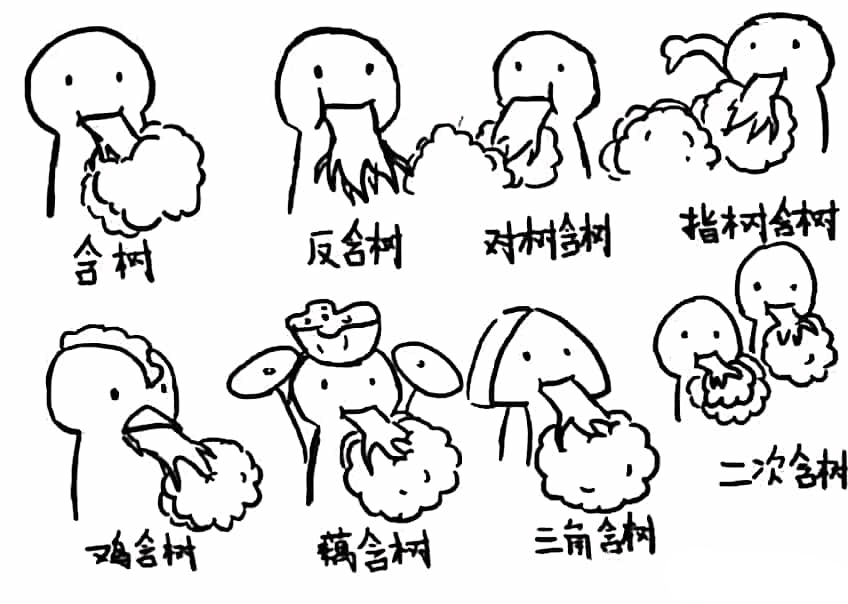
\includegraphics[scale=0.4]{1.jpg}
				
				\caption{图文无关}
			\end{figure}
		\subsection{数学}
			数学复习过程中,小知识点很多,尽量不要遗漏。因此,一轮复习对数学来说非常重要,必须检查所有知识点是否把握到位。
			
			考试时要减少低级错误的产生,不跳步。如果不放心就快速再算一遍。
			
			一个题没有思路时,试试把复杂的式子强行化简,或者把相关题目的所有知识点都罗列出来看是否有适用的工具。
			
			同时,各种题目如果没有思路,就按照一种方法硬算下去,总会有一些步骤分。而把一些特殊情况提出来讨论也可以获得步骤分,如参数为0、斜率为0、斜率不存在等情况。
			
			如果写出答案却没有令人信服的步骤,也会被扣掉不少的分。所以一定要把步骤写清楚,实在写不清楚,甚至是猜出答案的,可以通过答案倒推上一步来迷惑阅卷老师,或者画图解释你的观点。
			
			此外,数学的选择填空题有多种魔法可以解决,如特值法、画图法、排除法。因为它不需要写过程,所以很有可能得到分。
	%揣摩命题人意图、阅卷人
		\subsection{英语}
			首先是词汇量。到高三后期,很多“不认识”的单词实际上都是前面课本上标$\triangle$的单词,所以在复习时所有的单词都要过一遍,同时再把平时阅读中遇到的生单词积累下来,就可以达到可观的词汇量。
			
			此外,还需要学会认派生词。当遇到生词时,先想想它的一部分是否和学过的某个单词有些相像,然后再代入上下文看合不合理。
			
			语法填空的知识点一般都很容易,只要把常见的易错点都区分开就没什么问题。
			
			英语作文最重要的是字迹工整,最简单的字迹工整就是每个字母上下对齐。
			
			\begin{figure}[h]
				\centering
				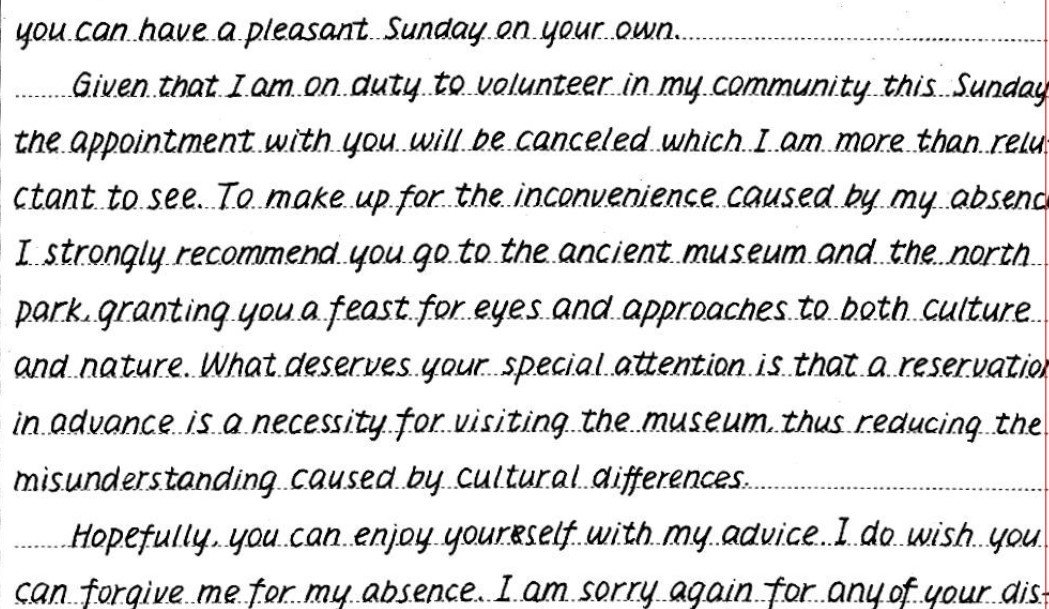
\includegraphics[width=16cm,height=9cm]{2.jpg}
				
				\caption{英语作文字迹写成这样就没啥问题了 from wjyyy}
			\end{figure}
		\subsection{物理}
			物理题目考察的主要是情景的建立。只需要脑子里模拟题设就能解决很多题目,剩下的就是计算了。我们同样也要记好每个公式、每个字母是什么含义。
			
			当然,物理题目也需要一定的文字说明,使阅卷老师知道你的分析和计算针对的是哪个物体。然后大量做题,形成“肌肉记忆”,才能提升做题速度。
		\subsection{化学}
			熟悉各类方程式和元素周期表,背下来老师要求背的东西即可。
			
			考试过程中一定要慢下来审题,题目中每一句话都是有用的,就算是迷惑信息也有它迷惑的价值。
			
			化学是一个极需要注意细节的学科,题目不难,但是需要较为完整的知识体系。例如,老高考的有机题,掌握以下知识点就没问题了。
			
			\begin{figure}[h]
				\centering
				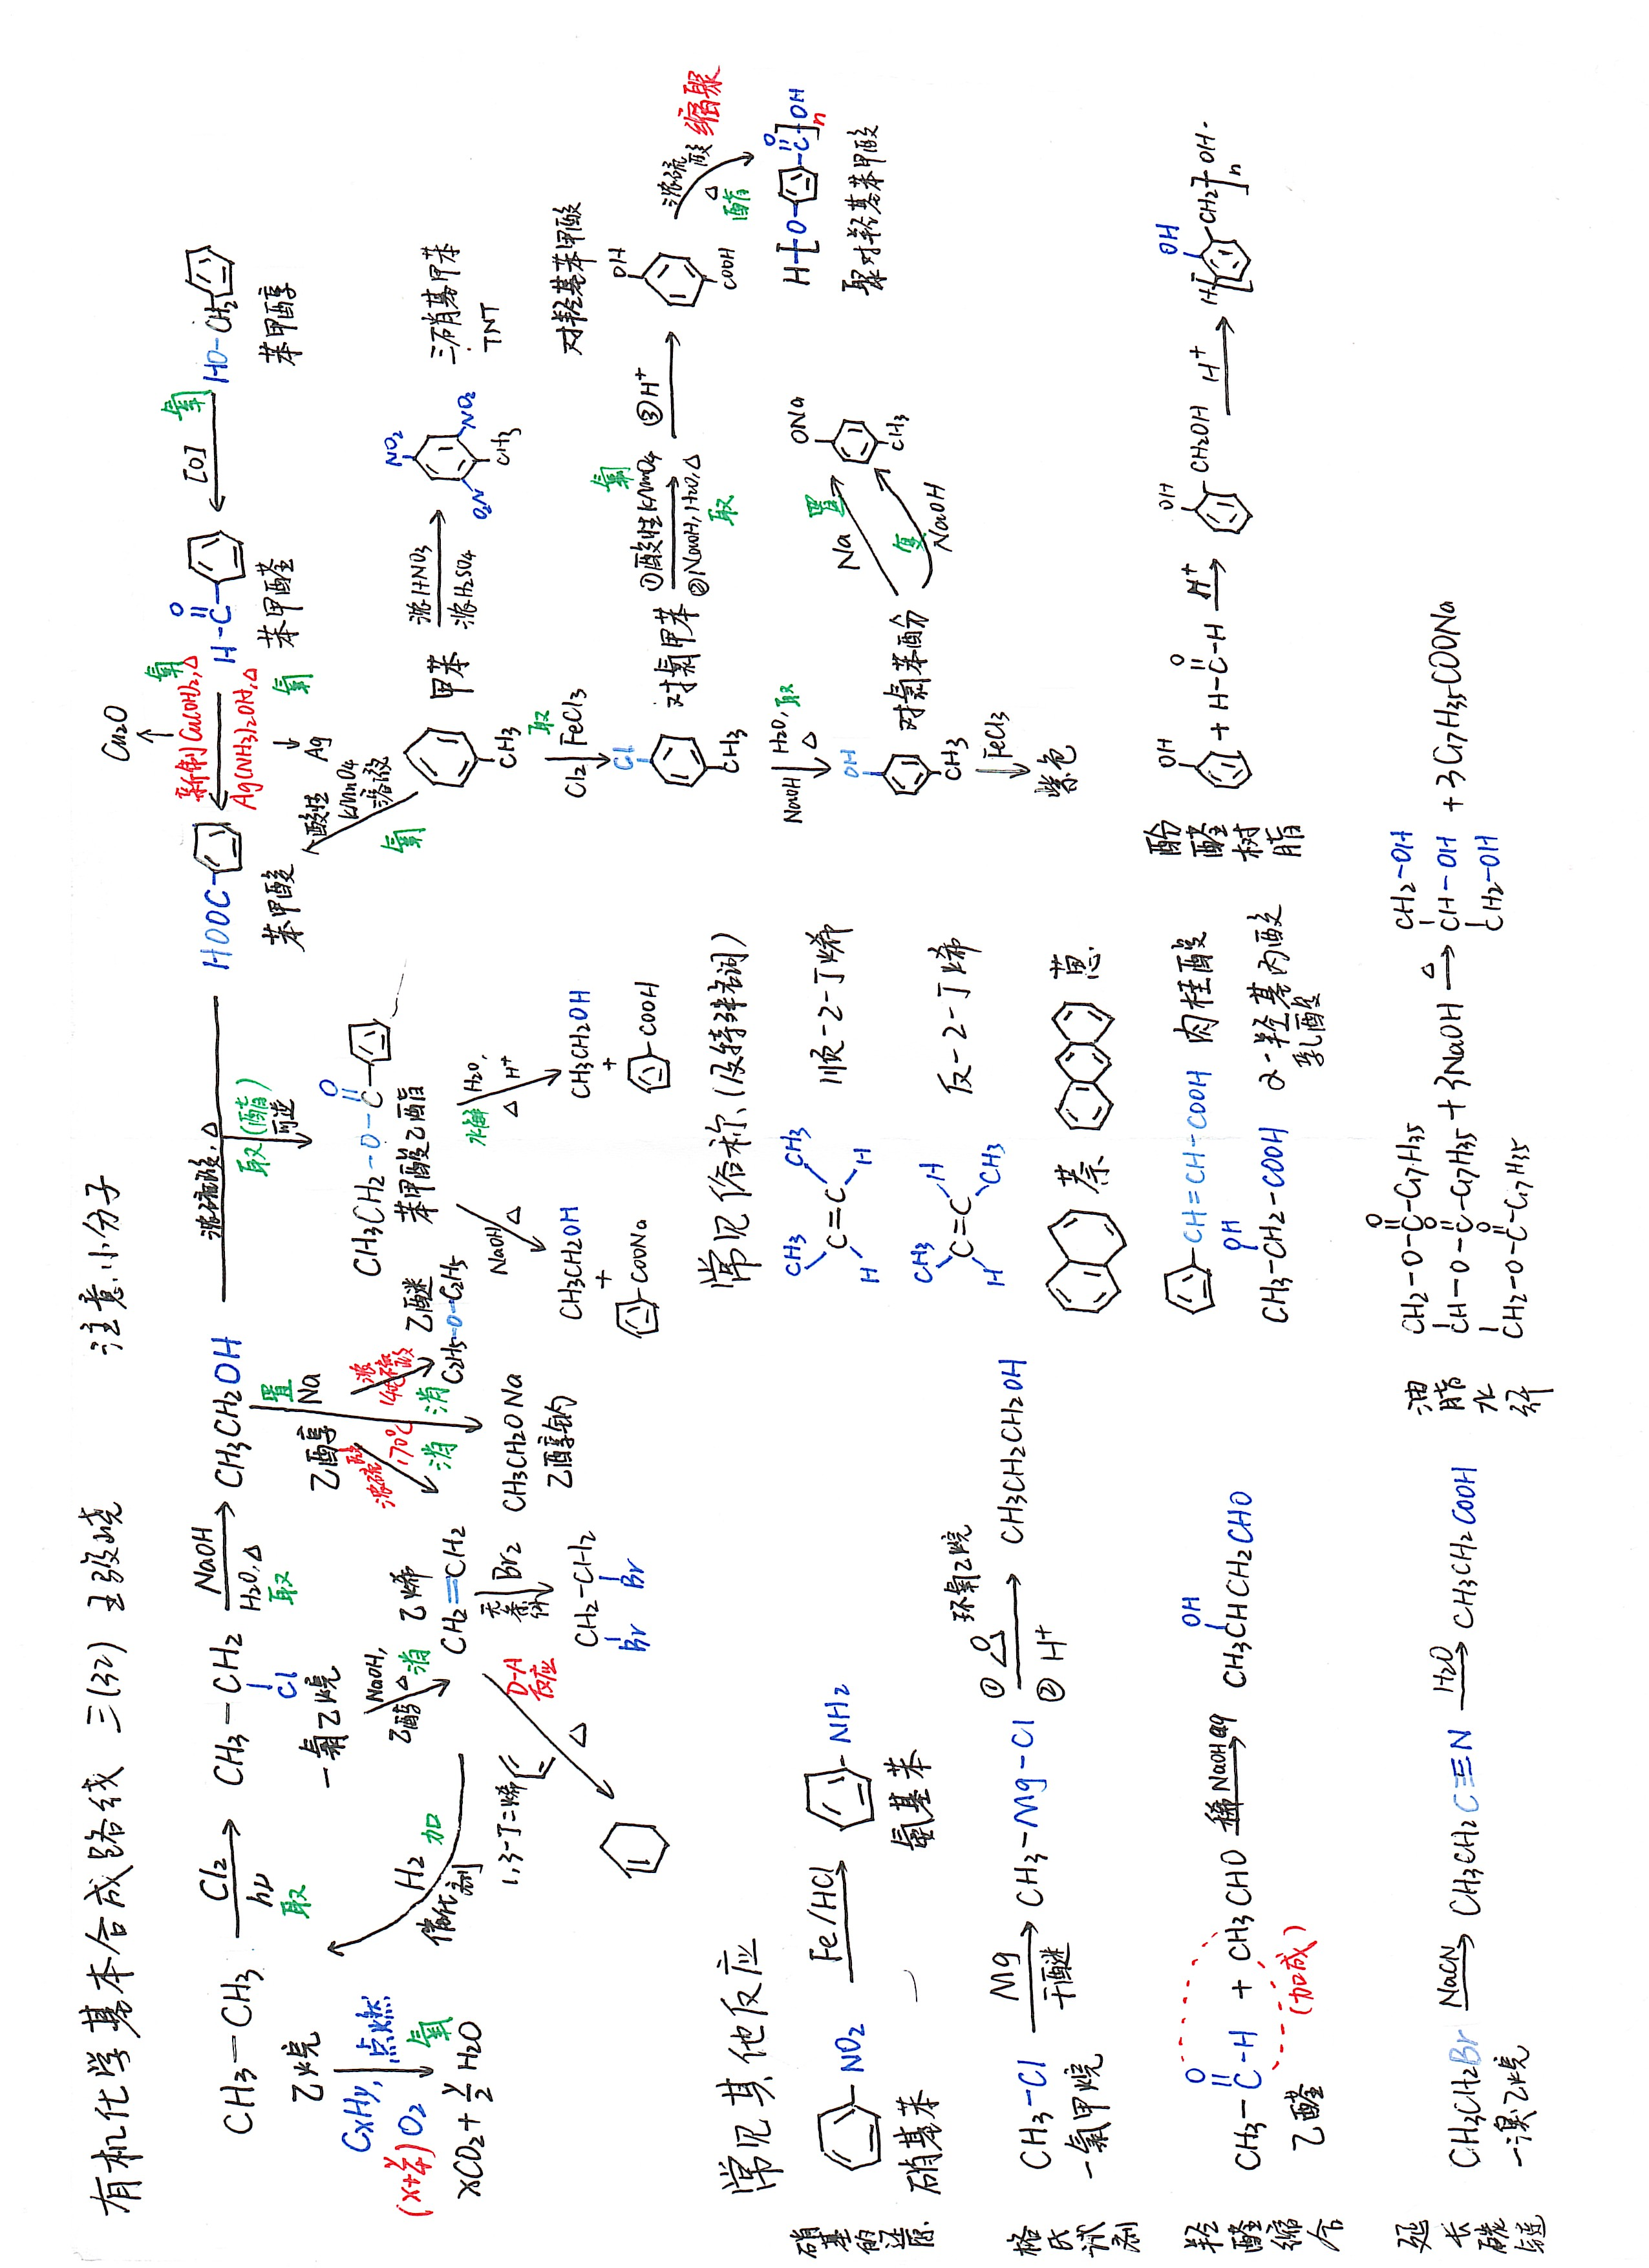
\includegraphics[width=10.5cm,height=16cm,angle=270]{2020-09-08_001.jpg}
				
				\caption{化学有机知识点融合}
			\end{figure}
		\subsection{生物}
			高中生物无非是\textbf{背知识点和做题}。做题的目的就是让知识点熟练。
			
			一个较明智的做法是在学习过程中就将课本中\textbf{黑体字}和笔记背一遍。
			
			生物也需要归纳总结,因为知识点过于零散。比如把所有颜色反应都放在一起比较,把遗传概率题放在一起分析,把所有细胞器和结构列个表等等。如果不会做的话可以去参考各大教辅资料的总结方式,再自己总结。
	\section{高三建议 - 态度}%乐观
		态度大体上可以分为生活态度和学习态度。生活态度决定了高三的心情等,学习态度则决定了最终的成绩。
		\subsection{生活态度}
			面对压力如山的高三,我们需要有乐观的态度和适当的调节能力。
			
			\begin{quote}
				\it 永远相信\\
				美好的事情即将发生\\
				\flushright{——小米}
			\end{quote}
		
			如果总是抱着“我不行”的态度,即使本来可以,最终也不太容易成功。
			
			如果总是觉得自己可以,就算本来不行,也有机会成功。
			
			其实,多一点自信,对生活没什么影响,态度却变得更加积极阳光了,也就更热爱生活。
			
			而偶尔的失利并不会打垮一个人,失利为我们带来的其实更多的是查漏补缺的机会。可能有时会觉得,这个漏洞太大了补不起来,那就慢慢找入手点,能补多少算多少。毕竟让一个人忙起来是使生活充实的最好方式。
		\subsection{学习态度}
			书写和卷面一定程度上表现了一个人的学习态度,因为它可以反映出这个人是否耐心。
			
			只要卷面整洁,字的大小相当,横平竖直,就可以基本满足高考的卷面需要了,毕竟老师改很多份试卷也会审美疲劳。
			
			在学校认真对待老师布置的任务,给老师留下较好的印象。比如勤找老师问问题、分析试卷。\sout{主要是混脸熟。}
			
			如果能力不是特别强,就最好听取老师的建议,老师一般不会给出错误的指引。
	\section{关于高考}
		高考是比较严格的,需要进行安检和各项保险工作,而且高考原则上是不能自带文具的,所以要尽快适应最普通的笔。
		
		高考没有那么难,因为平时对它的担心绝大部分都是不会出现的,而就是这种过量的担心导致了大家认为高考很难。
		
		两天,转瞬即逝。
			
	\section{其他想说的}
		上了高三以后,两天用一根笔是非常正常的。只要做题量不大,没有一天一根那么夸张。
		
		高中其实不怎么需要额外买资料,实在是学有余力可以多做总结,再有时间就去做做套卷和真题。因为大多数同学高中的时间都被老师给安排得满满当当。
		
		一轮复习很重要,这是最后一次能追上前面同学的机会了。
		
		任何时候都要稳扎稳打,尽量不要飘。
	\section{结语}
		不要担心。要在最昏暗的高三发出自己的光。
		
		\begin{quote}
		\it 砸在地上的汗水是真的,落在心上的泪水是真的\\
		它浇灌出来的果实也是真的。
		\end{quote}
		
		感谢 Dew 的审稿。
		\flushright{wjyyy}
		
		\flushright{2020年9月8日}
\end{document}